\documentclass[a4paper,11pt]{article}
\usepackage[T1]{fontenc}
\usepackage[utf8]{inputenc}
\usepackage{lmodern}
\usepackage{hyperref}
\usepackage[top=2cm, bottom=2cm, left=2cm, right=2cm]{geometry}
\usepackage{graphicx}
\usepackage{listings}
\usepackage{color}

\title{Implementation of a compiler for an imperative language\\IMP}
\author{Remy Detobel \& Denis Hoornaert}
 
\definecolor{codegreen}{rgb}{0,0.6,0}
\definecolor{codegray}{rgb}{0.5,0.5,0.5}
\definecolor{codepurple}{rgb}{0.58,0,0.82}
\definecolor{backcolour}{rgb}{0.95,0.95,0.92}
 
\lstdefinestyle{mystyle}{
    backgroundcolor=\color{backcolour},   
    commentstyle=\color{codegreen},
    keywordstyle=\color{magenta},
    numberstyle=\tiny\color{codegray},
    stringstyle=\color{codepurple},
    basicstyle=\footnotesize,
    breakatwhitespace=false,         
    breaklines=true,                 
    captionpos=b,                    
    keepspaces=true,                 
    numbers=left,                    
    numbersep=5pt,                  
    showspaces=false,                
    showstringspaces=false,
    showtabs=false,                  
    tabsize=2
}
 
\lstset{style=mystyle}

\begin{document}

\maketitle
\tableofcontents

\section{Introduction}

  The aim of project is to implement a compiler for a 'simple' imperative language named \textit{IMP}. Like any imperative programming language, \textit{IMP} is composed of mainstream features such as \textit{keywords} (\verb|if|, \verb|while|, ... statements), \textit{variables}, \textit{numbers} and \textit{comments}.
  The form of these features follows some defined rules~:
  \begin{itemize}
    \item a \textit{variable} is a sequence of alphanumeric characters that must start by a letter.
    \item a \textit{number} is a sequence of one or more digits.
    \item a \textit{comment} must start by the combination '\verb|(*|' and ends by the reversed combination '\verb|*)|'. 
  \end{itemize}
  The compilation scheme is generally divided in three main phases~: analysis, synthesis and optimisation. The phases are themselves composed of different steps. For instance, the analysis phase is composed of \textit{lexical analysing} step (or \textit{scanning}), a \textit{syntax analysing} step (or \textit{parsing}) and a \textit{semantic analysing} step as shown in fig.\ref{compilation_phases}. In this assignment, the focus is set on the \textit{analysis phase}.
  \begin{figure}[h]
    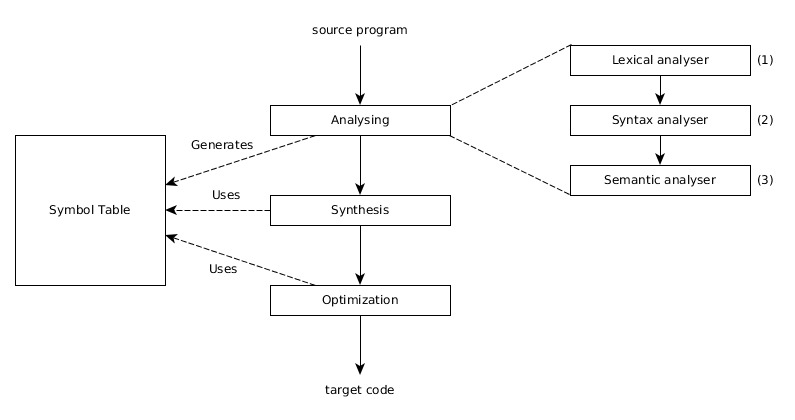
\includegraphics[scale=0.45]{./img/phase_of_compiler.jpg}
    \centering
    \caption{Compilation phases}
    \label{compilation_phases}
  \end{figure}
  
\section{Implementation of the lexical analyser}
  In the so called "Dragon book"\footnote{V. Aho, A., 2007. \textit{Compilers~: Principles, techniques, \& Tools.} 2nd ed. New York~: Pearson.} the \textit{lexical anlyser} is defined as follow~:
  \begin{center}
    <<The \textit{lexical analyser} reads the stream of characters making up the source program and groups the characters into a meaningful sequence called \textit{lexemes}.>>
  \end{center}
  A \textit{lexeme} can be defined as a tuple which contains both a \textit{token name} and the associated value (not always mandatory). The sequence of \textit{lexemes} generated by the \textit{lexical analyser} will be used by the following step. In addition, the \textit{lexical analyser} will generate a very useful tool used during all the other steps (as shown in fig.\ref{compilation_phases} .) and called a \textit{symbol table}. The role of the \textit{symbol table} is to store every variable encountered while scanning the source code and the line where it appears for the first time.\\
  
  \subsection{The use of a lexical analyser generator}
    In order to ease the process of recognizing the lexemes defined in the given \verb|LexicalUnits.java| file many \textit{lexical analysers} have been developed. Among them, the most well known generator is the flex program and all its derived versions. In the present project, \verb|jflex| is used as it has been decided to implement the project using the \verb|java| programming language. Using a \textit{lexical analyser generator} eases the analysis of any input because it enables the programmers to describe every \textit{regular expression} by using the \textit{Regex} writing convention and then to generate a \verb|.java| file that will recognise all of them. This generated \verb|.java| file can then be used as any other \verb|java| class.
    \begin{figure}[h]
      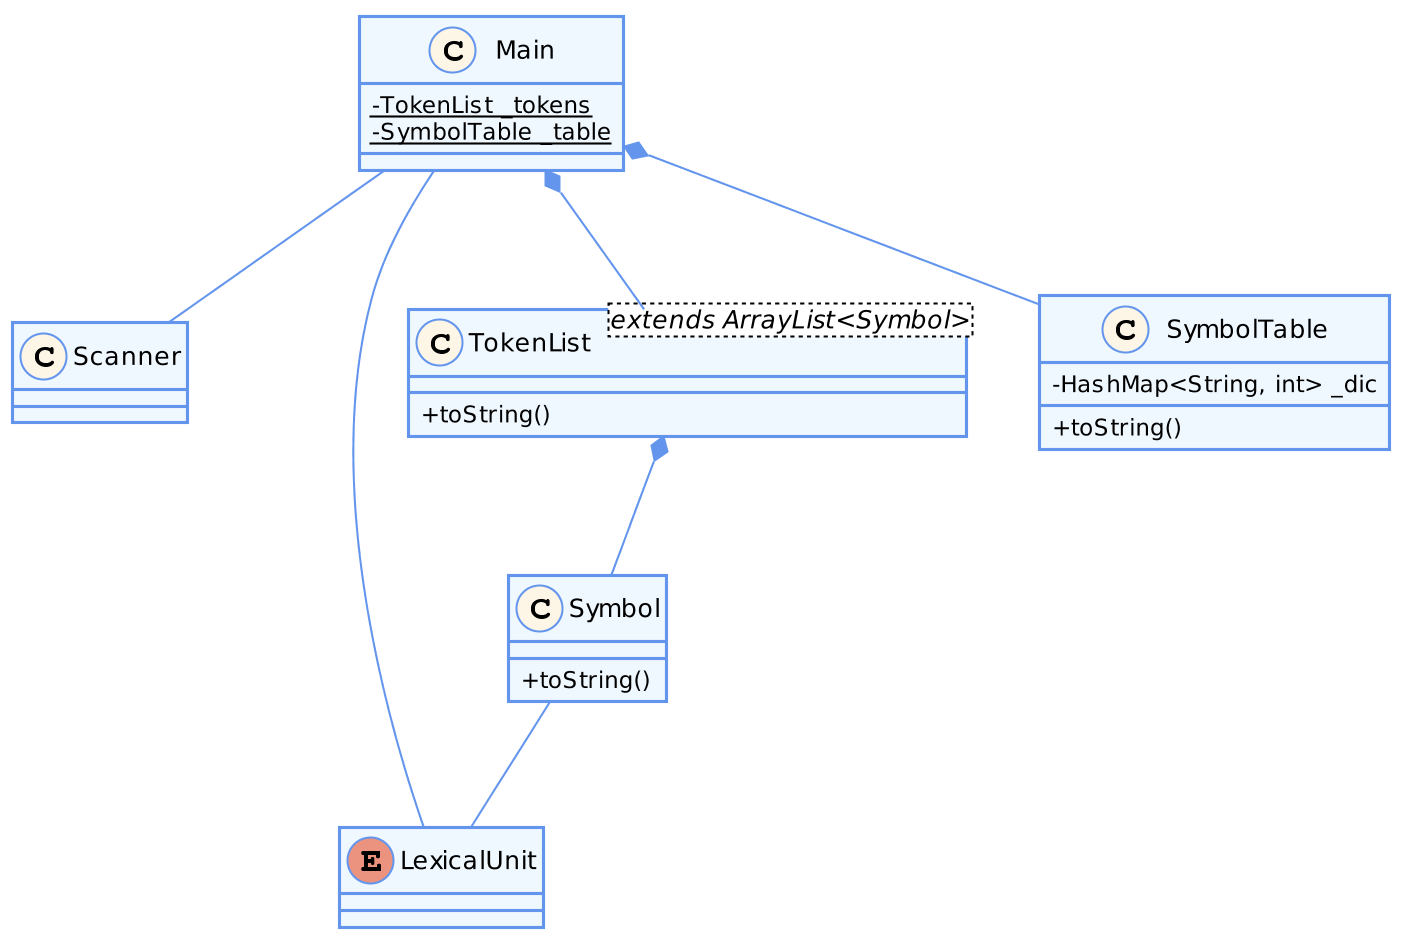
\includegraphics[scale=0.15]{./img/class_diag.png}
      \centering
      \caption{Model class (Pseudo-UML). The TokenList class is the sequence of lexemes and the Scanner class is the file generate by jflex}
    \end{figure}
  
  \subsection{Regular expressions}
    Based on the content of \verb|LexicalUnits.java|, we can easily divide the set of lexical units into two distinct groups~: the \textit{keyword} group and the variable/constant group.\\
    The implementation of the \textit{keyword} group using regular expressions is pretty straightforward as simply writing the \textit{keyword} is sufficient. For instance, the regular expression of the \textit{keyword} \verb|if| is simply \verb|if|.\\
    On the other hand, the implementation of the variable/constant group requires slightly more work. This small group is composed of two elements the variables and the numbers.\\
    The structure of \textit{variables} given in the assignment statements is "a sequence of alphanumeric characters that must start by a letter". Thus, the equivalent regular expression is~:
    \begin{verbatim}
[a-zA-Z][a-zA-Z0-9]*
    \end{verbatim}
    The structure of \textit{numbers} given in the assignment statements is "a sequence of one or more digits". thus, the equivalent regular expression is~:
    \begin{verbatim}
[0-9]+
    \end{verbatim}
  
  \subsection{Hypothesis on regular expressions}
    \label{hypothesis}
    The only hypothesis that has been made throughout the realisation of the project concerns the behaviour of the \textit{lexical analyser} when a character not specified in either the structure of a \textit{number}, a \textit{variable} or a \textit{keyword} is encountered. Typically, amongst this set there are the following characters~:
    \begin{center}
      \verb|}|, \verb|{|, \verb|_|, \verb=|=, \verb|&|, \verb|[|, \verb|]|, \verb|(|, \verb|)|
    \end{center}
    In order words, the question is~: What does the \textit{lexical analyser} do for the following line~:
    \begin{lstlisting}
index_of_loop := list[x]\end{lstlisting}
    Three ideas have been considered~:
    \begin{itemize}
      \item Considering these characters as a new lexical unit identified by the following regular expression (not exhaustive)~:
        \begin{verbatim}
SpecialChar = ["}", "{", "_", "|", "&", "[", "]", "(", ")"]
        \end{verbatim}
        The example above would be transposed by the \textit{lexical analyser} into the following token list~:
        \begin{verbatim}
token: index              lexical unit: VARNAME
token: _                  lexical unit: SPECIALCHAR
token: of                 lexical unit: VARNAME
token: _                  lexical unit: SPECIALCHAR
token: loop               lexical unit: VARNAME
token: :=                 lexical unit: EQUAL
token: [                  lexical unit: SPECIALCHAR
token: x                  lexical unit: VARNAME
token: ]                  lexical unit: SPECIALCHAR
        \end{verbatim}
        Unfortunately, the assignment statement disallows us to modify the \verb|LexicalUnits.java| file. Consequently, this possibility is not relevant.
      \item Considering these characters as normal characters. This would mean that they could be part of a \textit{variable} name. Thus, the regular expression for identifying \textit{variables} has to be modify to look like~:
        \begin{verbatim}
SpecialChar = ["}", "{", "_", "|", "&", "[", "]", "(", ")"]
[a-zA-Z|SpecialChar][a-zA-z0-9|SpecialChar]*
        \end{verbatim}
        As a consequence, the token list generated by the \textit{lexical analyser} will behave as follow~:
        \begin{verbatim}
token: index_of_loop      lexical unit: VARNAME
token: :=                 lexical unit: EQUAL
token: [x]                lexical unit: VARNAME
        \end{verbatim}
        Even though, using characters like \verb|_| in variable name is common in many programming languages, the other characters are generally not used for this purpose. Given this fact and the fact that the assignment statement does not explicitly mention such a possibility, this idea has been overlooked. Moreover, this implies that variable such as \verb|{{!^^§'#| would be considered as valid even though having such \textit{variables} is not handy.
      \item Not considering them. In this possibility, we just overlook them like if they were equivalent to a space character. This solution is the one who fits the best the assignment statements. Therefore, this solution has been preferred over the two others.
    \end{itemize}

  \subsection{Dealing with nested comments}
    The management of comments using regular language is quite simple. Once an opening statement (here : '\verb|(*|') has been encountered, it overlooks the following characters until it encounters a closing statement (here : '\verb|*)|').
    \begin{lstlisting}
(*I am a (*nested*) comment*)\end{lstlisting}
    Unfortunately, applying the same mechanism on a nested comment will result in a ill-formed outcome. Indeed, in the case of the example above, the analyser will overlook the second opening statement (columns 9 \& 10) and will stop when it comes across the first closing statement (columns 17 \& 18) having for consequence that the third part of the \textit{nested comment} will remain.\\
    To overcome this problem, the analyser must know how many opening statements it came across and how many closing statements it should expect to encounter in order to know whether it is still in a comment.\\
    The most obvious and smartest way to implement it is to use a counter (i.e. a memory) that will be incremented for every opening statement encountered and decreased for every closing statement encountered. However, from a theoretical point of view, by using a memory the language cannot be considered as regular any more. In the present project, it is not a problem and \verb|jflex| allows us to implement such a language.
    
\section{Tests and results}
  In this section, the results of the implementation are analysed and tested throught three \textit{IMP} source codes~: one given in the assignment statements and the two others inspired by algorithms from the Syllabus of Thierry Massart\footnote{Thierry Massart, 2014. \textit{Programmation.} Release 3.3.3~.}. The aim of testing the \textit{lexical analyser} on these three tests is to ensure that every \textit{keyword} and \textit{variable} is recognized because the set of keywords in the \verb|Euclid.imp| file does not cover every possibilities. This is why, even though the \textit{IMP} language does not handle lists, these two codes have been chosen. As explained above in the Hypothesis subsection \ref{hypothesis}, every unknown/undefined character is simply overlooked. Therefore, the \verb|[| and \verb|]| characters (which are generally used as operator on lists) does not trouble the lexical analysing.
  \begin{figure}[h!] % cacule réellement le gcd
    \lstinputlisting{../../test/Euclid.imp}
    \caption{\textit{IMP} code to compute the gcd of two numbers}
  \end{figure}
  \begin{figure}[h!] % "binary search" =?= "reherche dicotomique"
    \lstinputlisting{../../test/Search.imp}
    \caption{Implementation of a binary search using \textit{IMP}}
  \end{figure}
  \begin{figure}[h!]
    \lstinputlisting{../../test/Sort.imp}
    \caption{Implementation of a sorting algorithm using \textit{IMP}}
  \end{figure}  

\section{How to set up the project}
  In order to simplify the compilation and the support of external libraries, it has been decided to use a well known \textit{java} project manager named \textit{Maven}. Its configuration file (\verb|pom.xml|) defines the \verb|main| file, defines the source folder, manages the \textit{JFlex} library and the package that must be compiled with this library.
  \subsection{Compilation}
    Compiling the project with \textit{Maven} is easy as the user only needs to execute~: \verb|mvn clean compile|. However, at the first execution, the user needs to execute \verb|mvn install| so that \textit{Maven} can install the required library.\\
    If the user does not want to use \textit{Maven}, he can execute different commands from the root project~:
    \begin{verbatim}
java -jar jflex-1.6.1.jar -d src/be/ac/ulb/infof403/ src/be/ac/ulb/infof403/lex/Scanner.flex
    \end{verbatim}
    Where \verb|jflex-1.6.1.jar| is the path to the \verb|.jar| executable library,  \verb|-d| is the output folder path specifier and the last parameter is the path to the \verb|.flex| file.\\
    Then, the user can compile the java source codes and can create the corresponding \verb|.class| files. The bash command to compile all the \textit{java} files located in the \verb|src/| folder is the following~:
    \begin{verbatim}
javac -d target $(find ./src/* | grep .java)
    \end{verbatim}
    This command generates the corresponding \verb|.class| files and put them in the \verb|target/| folder. You must create the "target" folder if it does not currently exist. Finally, the \textit{jar} file can be generated by using the command~:
    \begin{verbatim}
jar cvfe dist/INFO-F403-IMP.jar be/ac/ulb/infof403/Main -C target/ .
    \end{verbatim}
    Where \verb|INFO-F403-IMP.jar| is the name of the generated \textit{jar} file and \textit{target} is the folder where are located the \verb|.class| files.
    
  \subsection{Execution}
    To execute the resulting jar file, the user only has to type~:
    \begin{verbatim}
java -jar dist/INFO-F403-IMP.jar <sourceFile>
    \end{verbatim}
    Where \verb|<sourceFile>| is the path to the IMP file. If the source file is not specified then the program will use the file \verb|test/Euclid.imp|.
    
  \subsection{Test}
    The program has a system which automatically compares each output file (\verb|.out|) to the result of the execution of the corresponding \verb|.imp| file. The execution of the test can be specified by adding the parameter \verb|-test| at the program execution instruction, like this~:
    \begin{verbatim}
java -jar dist/INFO-F403-IMP.jar <sourceFile> -test <testFile>\end{verbatim}
    Where \verb|<testFile>| is the name of the output file. If not specified, the program will automatically load a file test based on the \textit{source file} name. It will only change the file extension from \verb|.imp| to \verb|.out|.
    
    
  \subsection{Javadoc}
    The javadoc is located in the \verb|doc/| folder. To generate the javadoc with Maven you must execute \verb|mvn javadoc:javadoc|.  If you do not want to user Maven, you could execute the following command~:
    \begin{verbatim}
javadoc -d doc/javadoc/ -keywords -sourcepath src -subpackages be
    \end{verbatim}
    Where \verb|doc/javadoc/| is the output folder. The option \verb|-keywords| enable HTML in the javadoc.


\end{document}
